% Created 2024-10-03 Thu 21:47
% Intended LaTeX compiler: lualatex
\documentclass[presentation,professionalfonts,aspectratio=169]{beamer}
                

% 
\makeatletter
 \@ifclassloaded{beamer}{%
  %%% save beamer's `solution' environment as `beamersolution':
  \let\beamersolution\solution
  \let\endbeamersolution\endsolution
  %%% "delete" the `solution' environment:
  \let\solution\relax
  \let\endsolution\relax
}{%
}%
\makeatother
\usepackage[utf8]{inputenc}
\usepackage[T1]{fontenc}
%\usepackage[french]{babel}
\usepackage[portuguese]{babel}

%%%% FONTS




\usepackage{xsim}
\usepackage[most]{tcolorbox}
\usepackage{amssymb}
\usepackage{fontawesome}
\newcounter{paragraph}



\DeclareExerciseEnvironmentTemplate{custom}{%
  \begin{tcolorbox}[boxrule = 0pt]
  \tcbox[on line,colback=teal,colframe=teal,coltext=white,size=small]{%
    \faBook\sffamily\bfseries\
    \XSIMmixedcase{\GetExerciseName}
    \GetExerciseProperty{counter}%
  }\quad
}{\end{tcolorbox}}


\DeclareExerciseEnvironmentTemplate{custom2}{%
  \begin{tcolorbox}[boxrule = 0pt]
  \tcbox[on line,colback=violet,colframe=violet,coltext=white,size=small]{%
    \faToggleOn\sffamily\bfseries\
    \XSIMmixedcase{\GetExerciseName}
    \GetExerciseProperty{counter}%
  }\quad
}{\end{tcolorbox}}




\DeclareExerciseType{test}{
	exercise-env = question ,
	solution-env = answer ,
	exercise-template = custom ,
	solution-template = custom2 ,
	exercise-name	= Exemplo. ,
	exercises-name = Exemplo ,
	solution-name = Solução ,
	solutions-name = Sol. ,
	exercise-heading = \textbf ,
	solution-heading = \textbf
}


\xsimsetup{
  exercise/within = section,
  exercise/the-counter =  \arabic{exercise}, 
%%solution-name = solution,  % used with headings=true
solution/print=false,
%print-collection/print=both,
}





\usepackage{colortbl}
\usepackage[tikz]{bclogo}
\usetikzlibrary{fit,patterns,shadows.blur,shapes,mindmap}
\usetikzlibrary{arrows,calc,arrows.meta,decorations.markings,shapes.symbols}
\usetikzlibrary{decorations.pathreplacing, decorations.pathmorphing,calc,arrows,positioning}
\usepackage{tikzpeople}
\usepackage{qrcode,hyperref}
\usepackage{upgreek}
%\usepackage[version=4]{mhchem}
\usepackage{tabularray}


\NewTblrTheme{fancy}{
\SetTblrStyle{caption-tag}{font=\bfseries}
\SetTblrInner[tblr,longtblr]{rowsep=2.5pt}
\DefTblrTemplate{firsthead, middlehead,lasthead}{default}{} % <---
\DefTblrTemplate{contfoot-text}{normal}{\scriptsize\textit{Continued on the next page}}
\SetTblrTemplate{contfoot-text}{normal}
}






\usepackage{chemfig,chemmacros,elements,chemformula}
\chemsetup{modules={all}}
\chemsetup[redox]{pos=top,roman=false}
\chemsetup[redox]{pos=top}
\chemsetup{redox/sep=.5em}
\chemsetup[redox]{explicit-sign=true}
\NewChemPhase\lqdd{\(\ell\)}
\NewChemPhase\gr{grafite}
\NewChemPhase\reac{reação}
\NewChemState\Enthalpy{symbol=H,superscript=,unit=\kilo\joule}%
\usepackage{siunitx}
\setchemfig{fixed length=false, atom sep=2.5em, arrow offset=6pt, scheme debug=false}%,angle increment=30}
\renewcommand*\printatom[1]{\ensuremath{\mathsf{#1}}} % This line changes the font of the atoms to sans serif
%%%% QRCODE
\usepackage{pdfpages}
\usepackage{mol2chemfig}
\usepackage{subfig,caption}
\usepackage{wrapfig}
\usepackage{enumitem}
\setitemize{label=\usebeamerfont*{itemize item}%
\usebeamercolor[fg]{itemize item}
\usebeamertemplate {itemize item}}
\usepackage{array} % ajust colunm table
\usepackage{cancel}
\usepackage[controls]{animate}
\renewcommand{\CancelColor}{\color{red}}

%%%%%%%%%%%%%%%%%%% CONFIG TCOLORBOX 

\newtcolorbox{mybox}[2][]{boxsep=0.5em,left=0.5em,
colback=blue!5!white, colframe=blue!75!black,
fonttitle=\bfseries\sffamily,
colbacktitle=blue!85!red!60,enhanced,
attach boxed title to top left={yshift=-3mm,xshift=5mm},
title=#2,#1}

\newtcolorbox{myrule}[2][]{boxsep=0.5em,left=0.5em,
colback=green!5!white, colframe=blue!75!black,
fonttitle=\bfseries\sffamily,
colbacktitle=blue!85!red!60,enhanced,
attach boxed title to top left={yshift=-3mm,xshift=5mm},
title=#2,#1}


\newtcolorbox{myex}[2][]{boxsep=0.5em,left=0.5em,
  colback=yellow!5!white, colframe=blue!75!black, 
  fonttitle=\bfseries\sffamily,
  colbacktitle=blue!85!red!60,enhanced,
  attach boxed title to top left={yshift=-3mm,xshift=5mm},
  title=#2,#1}


 \definecolor{col1}{HTML}{FF7878}
 \definecolor{col2}{HTML}{51B5F8}
 \definecolor{col3}{HTML}{68E1AA}
 \definecolor{col4}{HTML}{B869EA}
 \definecolor{col5}{HTML}{FF5500}
 \definecolor{col6}{HTML}{FFF8E7}
 \definecolor{col7}{HTML}{FF9966}
 \definecolor{col8}{HTML}{9400D3}



\definesubmol\nobond{-[,0.2,,,draw=none]\scriptstyle\color{blue}}
\newcommand{\re}{\hspace{-1cm}}
\newcommand{\af}{\hspace{2cm}}

%%%% Config X sim for BEAMER
\makeatletter
\@ifclassloaded{beamer}{%
%%% save beamer's `solution' environment as `beamersolution':
\let\beamersolution\solution
\let\endbeamersolution\endsolution
%%% "delete" the `solution' environment:
\let\solution\relax
\let\endsolution\relax
}{%
}%
\makeatother
\usepackage[utf8]{inputenc}
\usepackage[T1]{fontenc}
%\usepackage[portuguese, ]{babel}
%%%% FONTS
%%% XSIM CONFIG BEAMER
\usepackage{xsim}
\usepackage[most]{tcolorbox}
\usepackage{amssymb}
\usepackage{fontawesome}
\usepackage{tasks}
\newcounter{paragraph}
%\usepackage[dvipsnames,svgnames]{xcolor}
\usepackage{xcolor}
\usepackage{annotate-equations}
%%% BOX EXERCISE BEAMER
\DeclareExerciseEnvironmentTemplate{custom}{%
\begin{tcolorbox}[boxrule = 0pt]
\tcbox[on line,colback=teal,colframe=teal,coltext=white,size=small]{%
\faBook\sffamily\bfseries\
\XSIMmixedcase{\GetExerciseName}
\GetExerciseProperty{counter}%
}\quad
}{\end{tcolorbox}}
%% == CUSTOM BOX BEAMER
\DeclareExerciseEnvironmentTemplate{custom2}{%
\begin{tcolorbox}[boxrule = 0pt]
\tcbox[on line,colback=violet,colframe=violet,coltext=white,size=small]{%
\faToggleOn\sffamily\bfseries\
\XSIMmixedcase{\GetExerciseName}
\GetExerciseProperty{counter}%
}\quad
}{\end{tcolorbox}}
\DeclareExerciseType{test}{
exercise-env = question ,
solution-env = answer ,
exercise-template = custom ,
solution-template = custom2 ,
exercise-name = Exemplo ,
exercises-name = Exemplo ,
solution-name = Solução ,
solutions-name = Sol. ,
exercise-heading = \textbf ,
solution-heading = \textbf
}
\xsimsetup{
exercise/within = section,
exercise/the-counter =  \arabic{exercise},
%%solution-name = solution,  % used with headings=true
solution/print=true,
print-collection/print=both,
}
\NewTasksEnvironment[label = (\emph{\alph*}),
label-width = 12pt]{choice}[\choice]
\usepackage{empheq} %%% Brackers
\usepackage{colortbl}
\usepackage[tikz]{bclogo}
\usetikzlibrary{fit,patterns,shadows.blur,shapes,mindmap}
\usetikzlibrary{arrows,arrows.meta,decorations.markings,shapes.symbols}
\usetikzlibrary{decorations.pathreplacing, decorations.pathmorphing,calc,arrows,positioning}
\usepackage{tikzpeople}
\usepackage{qrcode,hyperref}
\usepackage{upgreek}
%\usepackage[version=4]{mhchem}
\usepackage{tabularray}
%%% CUSTOM TABLE
\NewTblrTheme{fancy}{
\SetTblrStyle{caption-tag}{font=\bfseries,red2}
\SetTblrInner[tblr,longtblr]{rowsep=2.5pt}
\DefTblrTemplate{firsthead, middlehead,lasthead}{default}{} % <---
\DefTblrTemplate{contfoot-text}{normal}{\scriptsize\textit{Continua ...}}
\SetTblrTemplate{contfoot-text}{normal}
}
%% ==== CHEMMACROS E CHEMFIG CONFIG
\usepackage{chemfig,chemmacros,elements,chemformula}
\chemsetup{modules={all}}
\chemsetup[redox]{pos=top,roman=false}
\chemsetup[redox]{pos=top}
\chemsetup{redox/sep=.5em}
\chemsetup[redox]{explicit-sign=true} %%% reaction redox
%% == CUSTOM PHASES IN CHEMMACROS
\NewChemPhase\lqdd{\(\ell\)}
\NewChemPhase\gr{grafite}
\NewChemPhase\reac{reação}
\NewChemState\Enthalpy{symbol=H,superscript=,unit=\kilo\joule}%
\usepackage{siunitx}
\setchemfig{fixed length=false, atom sep=2.5em, arrow offset=6pt, scheme debug=false}
%% == NUMEROS PARA FORMULES
\renewcommand*\printatom[1]{\ensuremath{\mathsf{#1}}} % This line changes the font of the atoms to sans serif
%%% INCLUDE PAGES PDFs
\usepackage{pdfpages}
\usepackage{mol2chemfig}
\usepackage{subfig,caption}
\usepackage{wrapfig}
\usepackage{enumitem}
\setitemize{label=\usebeamerfont*{itemize item}%
\usebeamercolor[fg]{itemize item}
\usebeamertemplate {itemize item}}
\usepackage{array} % ajust colunm table
\usepackage{cancel}
\usepackage[controls]{animate}
\renewcommand{\CancelColor}{\color{red}}
%%%%%%%%%%%%%%%%%%% CONFIG TCOLORBOX
\newtcolorbox{mybox}[2][]{boxsep=0.5em,left=0.5em,
colback=blue!5!white, colframe=blue!75!black,
fonttitle=\bfseries\sffamily,
colbacktitle=blue!85!red!60,enhanced,
attach boxed title to top left={yshift=-3mm,xshift=5mm},
title=#2,#1}
\newtcolorbox{myrule}[2][]{boxsep=0.5em,left=0.5em,
colback=green!5!white, colframe=blue!75!black,
fonttitle=\bfseries\sffamily,
colbacktitle=blue!85!red!60,enhanced,
attach boxed title to top left={yshift=-3mm,xshift=5mm},
title=#2,#1}
\newtcolorbox{myex}[2][]{boxsep=0.5em,left=0.5em,
colback=yellow!5!white, colframe=blue!75!black,
fonttitle=\bfseries\sffamily,
colbacktitle=blue!85!red!60,enhanced,
attach boxed title to top left={yshift=-3mm,xshift=5mm},
title=#2,#1}
\definecolor{col1}{HTML}{FF7878}
\definecolor{col2}{HTML}{51B5F8}
\definecolor{col3}{HTML}{68E1AA}
\definecolor{col4}{HTML}{B869EA}
\definecolor{col5}{HTML}{FF5500}
\definecolor{col6}{HTML}{FFF8E7}
\definecolor{col7}{HTML}{FF9966}
\definecolor{col8}{HTML}{9400D3}
%% CONFIG COLOR CARBONO
\tikzstyle{bal}=[inner sep=0.3pt,fill=orange,fill opacity=0.5,circle,minimum size=0.2cm]
\tikzstyle{rect}=[inner sep=0.3pt,fill=red,fill opacity=0.5,circle,minimum size=0.2cm]
\tikzstyle{bal2}=[inner sep=0.3pt,fill=blue,fill opacity=0.5,circle,minimum size=0.2cm]
\tikzstyle{bal3}=[inner sep=0.3pt,fill=yellow,fill opacity=0.5,circle,minimum size=0.2cm]
\definesubmol\nobond{-[,0.2,,,draw=none]\scriptstyle\color{blue}}
\newcommand{\re}{\hspace{-1cm}}
\newcommand{\af}{\hspace{2cm}}
\date{}
%\usetheme{minflat}
\usetheme{minflat}
\author{Fábio Lima}
\date{}
\title{Funções Orgânicas Oxigenadas}
\hypersetup{
 pdfauthor={Fábio Lima},
 pdftitle={Funções Orgânicas Oxigenadas},
 pdfkeywords={},
 pdfsubject={},
 pdfcreator={Emacs 29.4 (Org mode 9.6.15)}, 
 pdflang={En Portuguese}}
\begin{document}

\begingroup
  \setbeamertemplate{headline}{}
  \maketitle
  \endgroup
\begin{frame}{Sumário}
\tableofcontents
\end{frame}





\section{Funções Oxigenadas}
\label{sec:org5f87523}
\begin{frame}[label={sec:org4d27bf5}]{Definição}
\begin{center}
\scalebox{.65}{
\begin{tikzpicture}[mindmap, grow cyclic, every node/.style=concept, concept color=orange!40, 
	level 1/.append style={level distance=5cm,sibling angle=35},
	level 2/.append style={level distance=2.8cm,sibling angle=90},]

	\node {Funções \\ Oxigendas}
	child {node [concept color = blue!40] {Álcoois}
	%	child {node [concept color = teal!30] {\chemfig{R-OH} \\ }}
	}
	child [concept color = blue!30] {node {Áldeído}
		%	child [concept color = teal!30, xshift=.5cm, yshift=1cm, text width=2.1cm,] {node {\chemfig{R-[:30](=[:90]O)-[:330]H}}}
	}
	child {node [concept color = blue!30] {Cetonas}
		%child [concept color = teal!30, xshift=.3cm, yshift=.3cm, text width=2.2cm] {node {\chemfig{R-[:30](=[:90]O)-[:330]R}  }}
	}
	child [concept color = blue!30] {node {Enol}
%		child [concept color = teal!30, xshift=.3cm, yshift=.3cm, text width=2.2cm] {node {\chemfig{R-[:30](-[:90]OH)=[:330]R}  }}
	}
	child [concept color = blue!30] {node {Éster}
	%			child [concept color = teal!30, xshift=1.5cm, yshift=1cm, text width=3.3cm] {node {\chemfig{R-[:30](=[:90]O)-[:330]O-R}}}
	}
	child [concept color = blue!30] {node {Éter}
		%		child [concept color = teal!30,xshift=.5cm, yshift=1cm, text width=2.5cm] {node {\chemfig{R-O-R}}}
	}
	child [concept color = blue!30] {node {Ácido \\ Carboxílico}
			%	child [concept color = teal!30, xshift=1.5cm, yshift=1cm, text width=3.cm] {node {\chemfig{R-[:30](=[:90]O)-[:330]OH}}}
	}
	child [concept color = blue!30] {node {Fenóis}
				%child [concept color = teal!30, xshift=.5cm, yshift=.5cm, text width=2.2cm] {node {\chemfig{**6(----(-OH)--)}  }}		
	}
	child [concept color = blue!30] {node {Sais \\ Orgânicos}
				%child [concept color = teal!30, xshift=1.5cm, yshift=1cm, text width=3.cm] {node {\chemfig{R-[:30](=[:90]O)-[:330]O-Metal}}}
	}
	child [concept color = blue!30] {node {Anidridos}
				%child [concept color = teal!30, xshift=1.5cm, yshift=.3cm, text width=4.2cm] {node {\chemfig{R-[:150](=[:90]O)-[:210]O-[:150](-[:210]R)=[:90]O}}}
};
	
\end{tikzpicture}
}
\end{center}
\end{frame}




\section{Álcool}
\label{sec:org8e9583b}
\begin{frame}[label={sec:org5f72865}]{Álcool}
\begin{mybox}{Álcool}
Substâncias  orgânicas  que  apresentam  hidroxila  ou oxidrila (-OH) ligada ao C saturado (\(sp^3\)).


  \begin{center}
% \chemfig{-C([:-90]-)([:90]-)-{\color{red}OH}}
\chemfig{-C([:90]-)([:-90]-)-[@{b1,0}]{\color{red}O}@{H}{\color{red}H}}
%\chemfig{C(-[2]H)(-[4]H)(-[6]H)-C(-[2]H)(-[6]H)-[@{b1,0}]O@{H}H}
\chemmove{
	\draw[-,magenta]
	(b1) -- ++(0,.45) -| (H.east)
	(b1) -- ++(0,-.45) -| (H.east) ;
}
Grupo Funcional
 \end{center}

\end{mybox}
\end{frame}


\begin{frame}[label={sec:org11d4d68}]{Fórmulas}
\begin{columns}
\begin{column}{0.45\columnwidth}
\begin{block}{Etanol}
\begin{center}
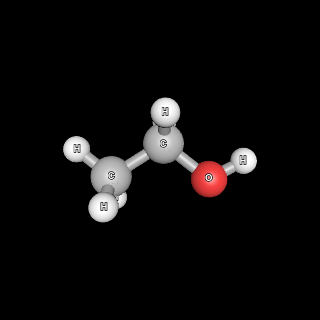
\includegraphics[scale=.5]{QO/FuncoesOxigenadas/Ethanol.png}
\end{center}
\end{block}
\end{column}



\begin{column}{0.45\columnwidth}
\begin{block}{Etanol}

    
\begin{center}
\chemfig{H_3C-[:30,,2]-[:330]O-[:30]H}
\end{center}


\scriptsize{
\begin{tblr}{lc}
Fórmula química & 	\ch{C2H6O} \\
Massa molar & 	46.06 \unit{\gram\per\mol}\\
Aparência  &	líquido sem cor\\
{Densidade\\ (Massa Específica 20°C)} & 0,789 \unit{\gram\per\cubic\centi\metre}\\
Ponto de fusão & −114.18 °C, 159 K, -174 °F\\
Ponto de ebulição & 	78.25 °C, 351 K, 173 °F\\
\end{tblr}
}
\end{block}
\end{column}
\end{columns}
\end{frame}



\begin{frame}[label={sec:orgbe7cd5a}]{Aplicações}
\end{frame}





\section{Enol}
\label{sec:org45b6a61}
\begin{frame}[label={sec:orgfdd41aa}]{Enóis}
\begin{mybox}{Enol}
Substâncias  orgânicas  que  apresentam  hidroxila  ou oxidrila (-OH) ligada ao C com uma dupla ligação.


  \begin{center}
\schemestart
\chemfig{-@{OH1}C([:90]-)([:-90]-)=C([:90]-)([:-90]-)-O@{OH2}H}
\schemestop
\chemmove{
	\node[inner sep=2pt,fill=red,fill opacity=0.2,fit=(OH1) (OH2)]{};
    }
    \end{center}

\end{mybox}
   \begin{myex}{Exemplo}
 \begin{center}  
 %  \chemname{
%   \chemfig{H_3{\color{red}C}-OH}}{{\color{red}Met}anol}\hspace{1cm}
   \chemname{
   \vspace{.3cm}
\chemfig{
           \mcfleft{\mcfatomno{4}}{C}H_3% 4
     -[:0]\mcfabove{C}{\mcfatomno{3}}H_2% 3
    -[:0]\mcfabove{C}{\mcfatomno{2}}H% 2
     =[:0]\mcfabove{C}{\mcfatomno{1}}H% 1
    -[:0]OH}% 
}
{But-1-en-1-ol}
\end{center}
%
\end{myex}
\end{frame}



\section{Fenol}
\label{sec:org310d26b}
\begin{frame}[label={sec:org5b1f0eb}]{Fenóis}
\begin{mybox}{Fenol}
Substâncias  orgânicas  que  apresentam  hidroxila  ou oxidrila (-OH) ligada ao carbono do anel aromático.



\begin{tikzpicture}
\tcbox[enhanced,sharp corners,colback=red!10,colframe=red]{\chemfig{*6(-=-=-(-OH)=-)}} \af
\tcbox[enhanced,sharp corners,colback=red!10,colframe=red]{\chemfig{**6(-----(-OH)--)}} \af
\end{tikzpicture}
\end{mybox}
\end{frame}

\begin{frame}[label={sec:org3d8c542}]{Tipos de fénois}
\begin{center}
\small
\centering
\chemname{\chemfig{*6(-=(-OH)-=-=)}}{Hidroxi Benzeno} \qquad  
\chemname{\chemfig{**6(---(**6(------))---)}}{Naftaleno} \\
\chemname{\chemfig{**6(--(**6(-**6(------)-----))----)}}{Antraceno}
\end{center}
\end{frame}


\section{Aldeídos}
\label{sec:org0cfcdac}
\begin{frame}[label={sec:org464edae}]{Aldeídos}
\begin{mybox}{Aldeído}
Os aldeídos apresentam o grupo carbonila na extremidade da cadeia.   


   \begin{center}
\begin{tikzpicture}
\tcbox[enhanced,sharp corners,colback=red!10,colframe=red]{\chemfig{R-C([:60]=O)([:300]-H)}} \hspace{.3 cm}
%\tcbox[enhanced,sharp corners,colback=red!10,colframe=red]{\chemfig{**6(-----(-OH)--)}}
\end{tikzpicture}
\end{center}
\end{mybox}
\end{frame}


\begin{frame}[label={sec:org4ec7605}]{Exemplos de Aldeídos}
\begin{columns}
\begin{column}{0.45\columnwidth}
\begin{block}{Metanal}
\begin{description}
\item[{Metanal (Formaldeído):}] Conhecido como formol, o aldeído fórmico, de fórmula estrutural CH2O, é utilizado na fabricação de desinfetantes e plásticos. Ademais, é importante no desenvolvimento de estudos científicos, uma vez que serve para conservação de cadáveres (fluido de embalsamamento).
\end{description}
\end{block}
\end{column}


\begin{column}{0.45\columnwidth}
\begin{block}{Metanal}
\begin{center}
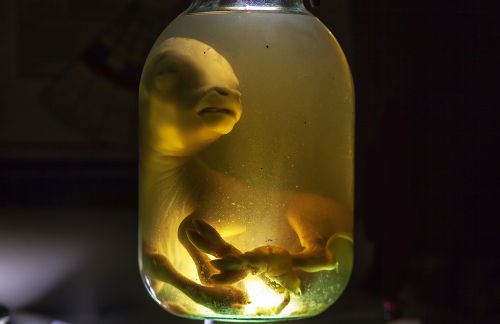
\includegraphics[width=.9\linewidth]{QO/FuncoesOxigenadas/formol.jpg}
\end{center}
\end{block}
\end{column}
\end{columns}
\end{frame}



\begin{frame}[label={sec:orga314ac5}]{}
\begin{columns}
\begin{column}{0.45\columnwidth}
\begin{block}{Aldeido}

\chemname{\chemfig{*6(-=-(-[:30]=[:-30]-([:90]=O)([:-30]-H))=-=)}}{Cinamaldeído}
\end{block}
\end{column}


\begin{column}{0.45\columnwidth}
\begin{block}{Aldeido}
\begin{center}
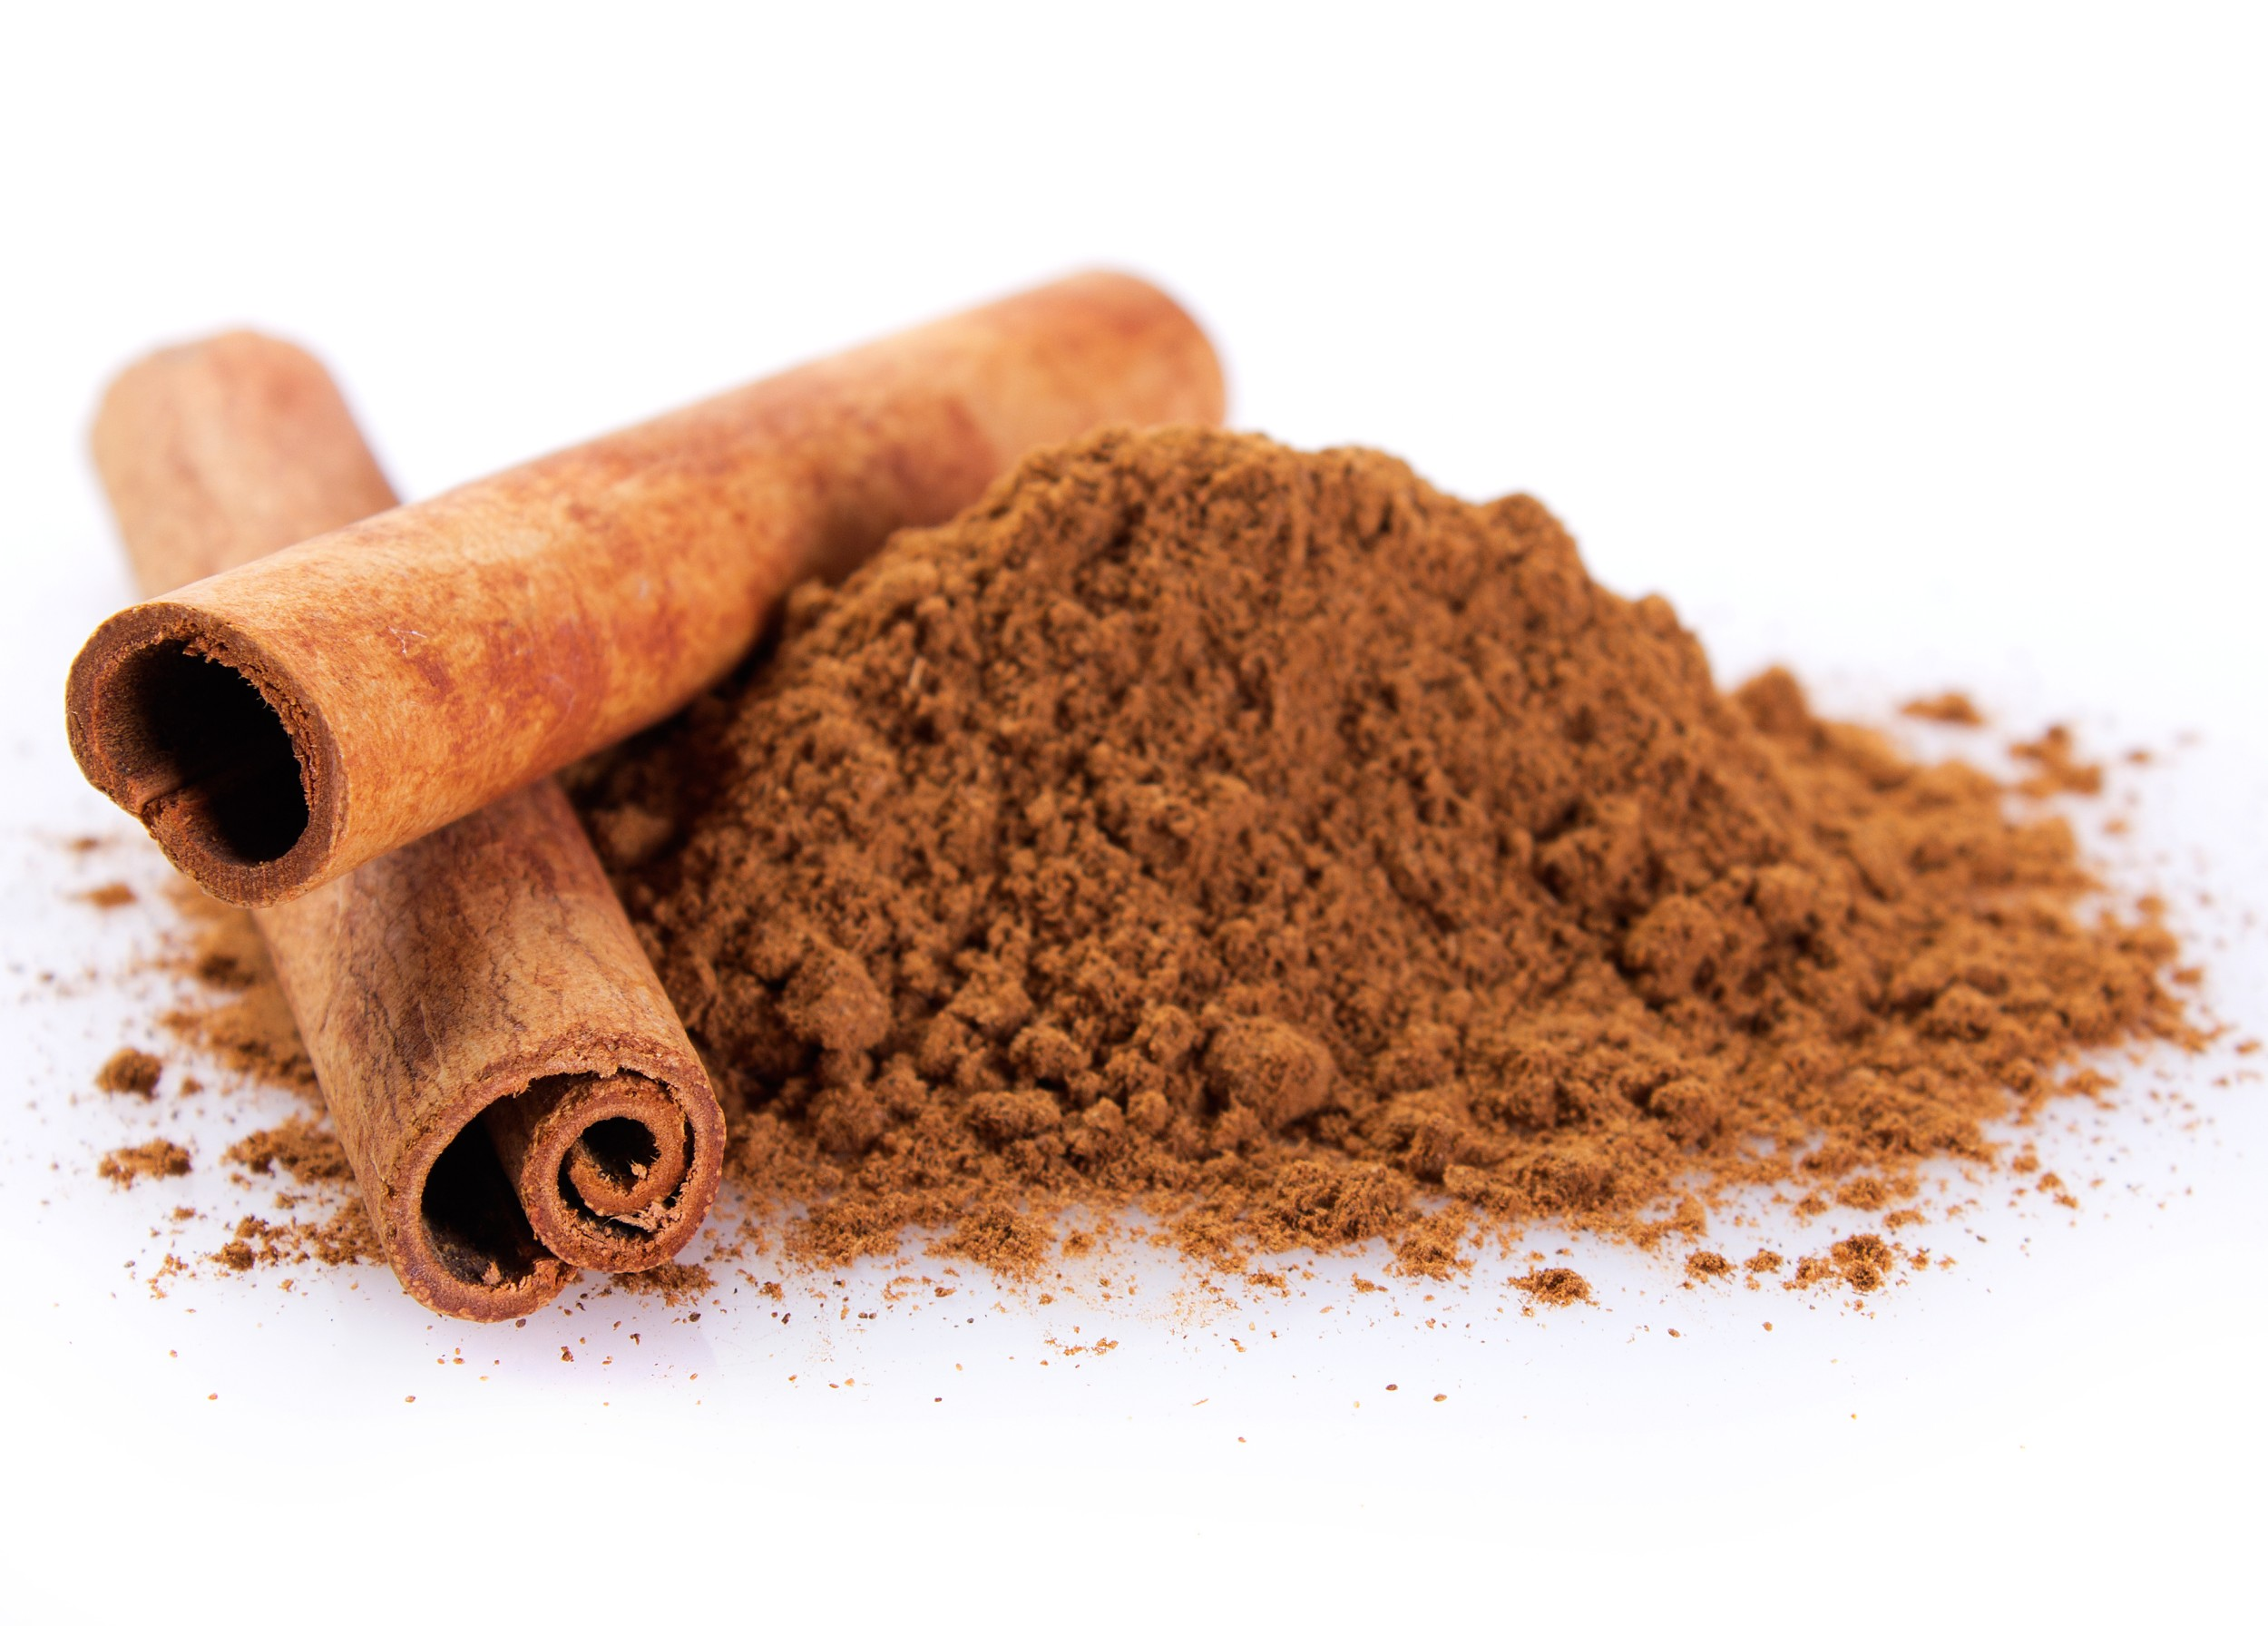
\includegraphics[width=.9\linewidth]{QO/FuncoesOxigenadas/canela.jpg}
\end{center}
\end{block}
\end{column}
\end{columns}
\end{frame}


\section{Cetonas}
\label{sec:orgf3f9ec7}

\begin{frame}[label={sec:org3ec9742}]{Cetonas}
\begin{mybox}{Cetonas}
As cetonas apresentam o grupo carbonila,sendo este carbono secundário.
\begin{center}
\begin{tikzpicture}
\tcbox[enhanced,sharp corners,colback=red!10,colframe=red]{\chemfig{R-C([:90]=O)-R}} \hspace{.3 cm}
\end{tikzpicture}
\end{center}
\end{mybox}
\end{frame}



\begin{frame}[label={sec:org9d5afbb}]{Propriedades Cetonas}
\begin{center}
\chemfig{H_3C-[:30,,2](-[:330,,,1]CH_3)=[:90]O}
\end{center}


\begin{itemize}
\item As cetonas possuem o grupo carbonila como grupo funcional.
\item A carbonila das cetonas deve estar ligada a outros átomos de carbono, não podendo estar na extremidade da cadeia.
\item As cetonas podem ser tanto de cadeia aberta quanto de cadeia fechada.
\item Toda cetona possui sufixo -ona em sua nomenclatura oficial.
\item O grupo carbonila aumenta o caráter polar das cetonas.
\item A propanona, vendida como acetona, é amplamente utilizada com solvente e removedora de tinta e esmalte.
\item As cetonas podem ser utilizadas na fabricação de perfumes e demais cosméticos devido a sua fragrância agradável.
\end{itemize}
\end{frame}




\section{Ácido Carboxílicos}
\label{sec:orgfad0c39}
\begin{frame}[label={sec:orgfdf971f}]{Ácidos Carboxílicos}
\begin{mybox}{Ácidos Carboxílicos}
Os ácidos carboxílicos são compostos caracterizados pela  presença do grupo \alert{carboxila}, formado pela união dos grupos carbonila e hidroxila.


\begin{center}
\begin{tikzpicture}
\tcbox[enhanced,sharp corners,colback=red!10,colframe=red]{\chemfig{-C([:30]=O)([:330]-OH)}} \hspace{.3 cm}
\end{tikzpicture}
\end{center}
\end{mybox}
\end{frame}


\section{Ésteres}
\label{sec:org0364133}
\begin{mybox}{Ésteres}
Os ésteres orgânicos são caracterizados pelo grupo funcional:
\begin{center}
\begin{tikzpicture}
\tcbox[enhanced,sharp corners,colback=red!10,colframe=red]{\chemfig{R-C([:90]=O)-O-R'}} \hspace{.3 cm}
\end{tikzpicture}
\end{center}
Simplificadamente podemos considerar queos ésteres
se originam a partir da substituição do hidrogênio do grupo OH de um
ácido carboxílico por um radical orgânico (R).
\end{mybox}


\section{Éteres}
\label{sec:org84734c2}

\begin{frame}[label={sec:org65d58a5}]{Éteres}
\begin{mybox}{Éteres}
Os éteres apresentam um átomo de oxigênio(O) ligado a dois radicais orgânicos.
Seu grupo funcional é representado por:

\begin{center}
\begin{tikzpicture}
\tcbox[enhanced,sharp corners,colback=red!10,colframe=red]{\chemfig{R-O-R'}} \hspace{.3 cm}
\end{tikzpicture}
\end{center}

\end{mybox}
\end{frame}





\section{Anidridos}
\label{sec:orge732d56}

\begin{frame}[label={sec:org99fe7ac}]{Anidridos}
\begin{mybox}{Anidridos}

Os anidridos orgânicos são compostos derivados de reações de desidratação dos ácidos carboxílicos. Daí a origem de seu nome, pois \alert{anhydros}, em grego, significa “ \alert{sem água} ”.


   \begin{center}
\schemestart
\chemfig{R-C([:60]=O)([:300]-@{a1}OH@{a2})} \+
\chemfig{[:180]R-C([:120]=O)([:240]-@{a3}H@{a4}O)}
\arrow
\chemfig{R-C(=[::+60]O)-[::-60]O-[::-60]C(=[::+60]O)-[::-60]R} \+ \chemfig{H_2O}
\schemestop
\chemmove{
\node[draw, blue, inner sep=1.3pt, fit=(a1) (a3)](quadro){};
\node[below=.8cm of quadro, ](text) {Desidratação Intermolecular};
\draw[>-Stealth] (quadro)--(text){};
}
 \end{center}

\end{mybox}
\end{frame}
\end{document}
